\documentclass{article}

% Language setting
% Replace `english' with e.g. `spanish' to change the document language
\usepackage[french]{babel}
\usepackage[fleqn]{amsmath} % Aligner les équations à gauche


% Set page size and margins
% Replace `letterpaper' with`a4paper' for UK/EU standard size
\usepackage[letterpaper,top=2cm,bottom=2cm,left=3cm,right=3cm,marginparwidth=1.75cm]{geometry}

% Useful packages
\usepackage{amsmath}
\usepackage{graphicx}
\usepackage{subcaption}
\usepackage[colorlinks=true, allcolors=blue]{hyperref}

\title{TD6}
\author{IPESUP - PC } 
\date{13 décembre 2023}

\begin{document}
\maketitle



\section{Mouvement d'une perle sur une tige en rotation}

Une petite perle, qu'on assimilera à un point matériel M, glisse sans frottement sur une tige horizontale (axe $Ox$) tournant à vitesse constante  $\omega _0$ autour de la verticale ($Oz$) . La perle est liée au
point $O$ par un ressort de raideur $k$ et de longueur à vide $l_0$. À l’instant initial,
le ressort n’est ni comprimé ni tendu et la perle a une vitesse nulle par rapport à la tige.
\\
On note $\omega ^2 = \frac{k}{m}$ et $a=\frac{\omega}{\omega _0}$


\begin{figure}[h]
  \centering
  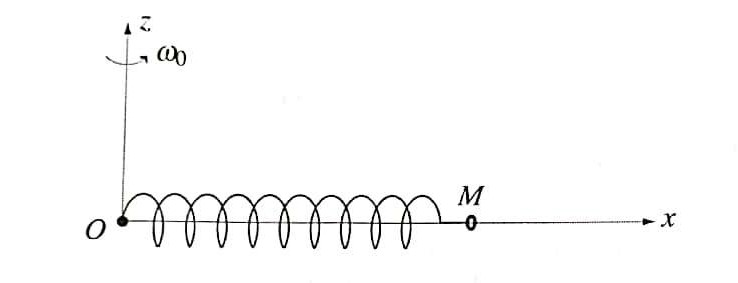
\includegraphics[width=0.45\textwidth]{ressort.jpg}
  \label{fig:maison}
    \caption{Schéma du ressort}
\end{figure}


\begin{enumerate}
    \item Etablir les équations du mouvement. 
    \item La figure 2 donne l'allure de la trajectoire de la perle pour différentes valeurs de a. Donner les conditions sur $a$ pour obtenir chacune des trois allures. On supposera désormais qu'on a $a>1$ 

\\[0.1cm]

\begin{figure}[h]
  \centering
  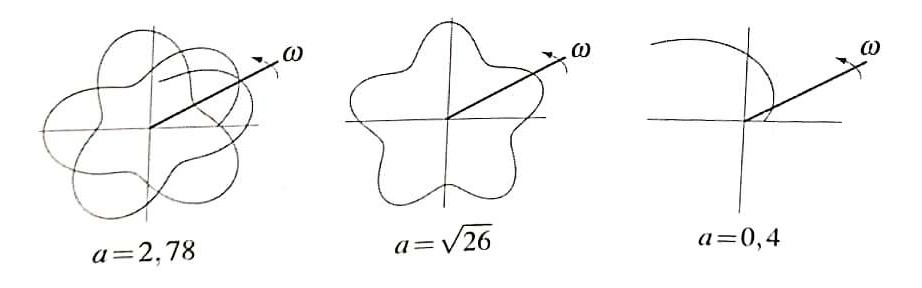
\includegraphics[width=0.45\textwidth]{fleurs.jpg}
  \label{fig:maison}
    \caption{Trajectoires possibles de la perle}
\end{figure}

\\[0.1cm]


\item Montrer que le ressort est toujours tendu
\item Déterminer la force exercée par la tige sur la perle
    
\end{enumerate}

\section{ Etude d'un sismographe}

Le sismographe vertical, représenté figure 3, est constitué d’une masse $m$ suspendue à
un ressort dont l’autre extrémité $\Omega$ est liée à un bâti rigide solidaire du sol en vibration. Un
dispositif d’acquisition permet d’enregistrer le mouvement de la masse m par rapport au bâti.
On souhaite que ce mouvement reproduise le plus fidèlement possible celui du sol par rapport
au référentiel d’étude $\mathcal{R}$ supposé galiléen. On appelle $\mathcal{R_S}$ le référentiel lié au bâti rigide
Le sol est supposé horizontal. Son mouvement vertical est décrit par une vibration de la
forme : $Z_s(t)= Z_0 cos(\omega t ).$ \\ 
Le ressort, de masse négligeable, de constante de raideur $k$, de longueur au repos $L_0$, a pour
longueur $L(t)$ à l’instant $t$. Un amortisseur relié au ressort, exerce sur la masse $m$ une action
mécanique modélisée par la force : $\vec{f_r}=-\lambda \vec{v}_{ / \mathcal{R_S}} (M) $ , où $\vec{v}_{ / \mathcal{R_S}} (M) $ est la vitesse de la masse
m dans le référentiel $\mathcal{R_S}$. 

\begin{figure}[h]
  \centering
  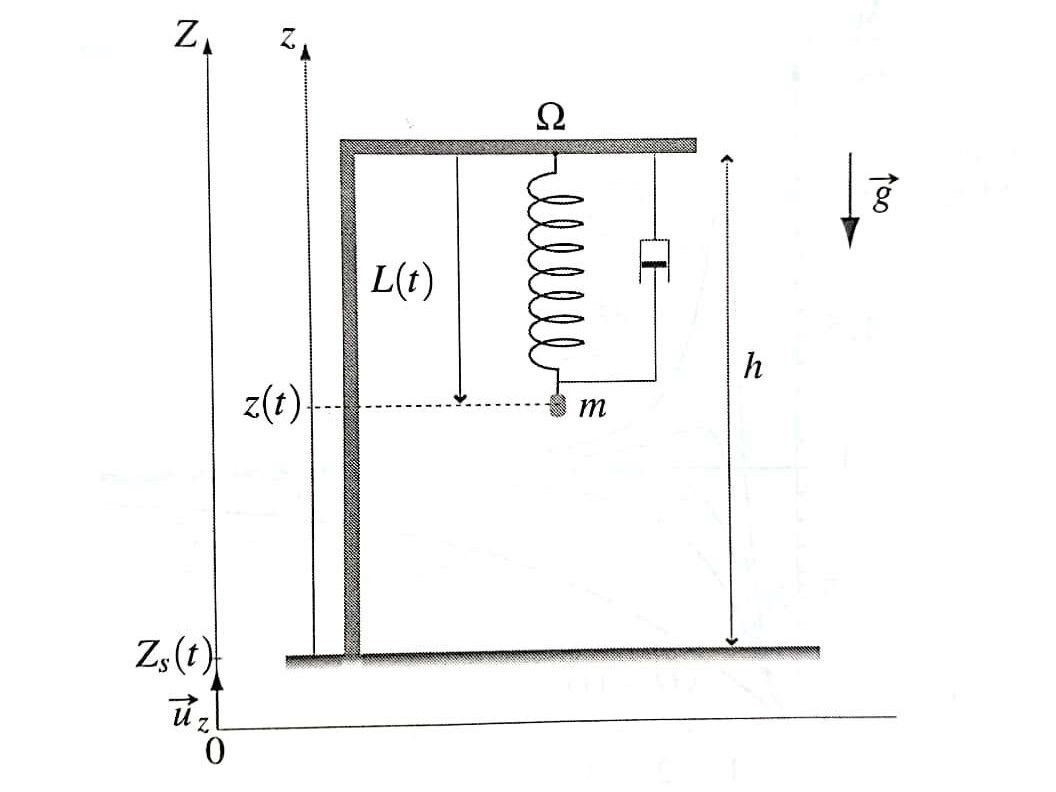
\includegraphics[width=0.45\textwidth]{sismographe.jpg}
  \label{fig:maison}
    \caption{Schéma d'un sismographe simple}
\end{figure}


On note $L_1$ la longueur du ressort quand la masse $m$ est à l’équilibre en l’absence de secousse
sismique. La masse $m$ se situe alors à la cote $z$ repérée par rapport au bâti. On repère dans la
suite la position de la masse $m$ par : $x(t) = z(t) - z_1$, où $z(t)$ est également repéré par rapport
au bâti du sismographe. 

\begin{enumerate}
    \item Établir l’équation différentielle vérifiée par $x(t)$ lors d’un séisme. L’écrire sous la forme : 

        
\begin{center}

   $ 
        \frac{d^2 x }{dt^2} + \frac{\omega _0}{Q} \frac{dx}{dt} + \omega _0 ^2 x = \omega ^2 Z_0 cos(\omega t)$
    
\end{center}


Donner les expressions de  $\omega _0$ et $Q$. 

        

On cherche la réponse du sismographe sous la forme : $x(t) = X_0 cos(\omega t + \phi)$. En posant :
$u=\frac{\omega}{\omega _0}$, montrer que : 




\begin{center}

   $ 
       \frac{X_0}{Z_0}=\frac{u^2}{\sqrt{(1-u^2)^2 + \frac{u^2}{Q^2}}}$
    
\end{center}

\begin{figure}[h]
  \centering
  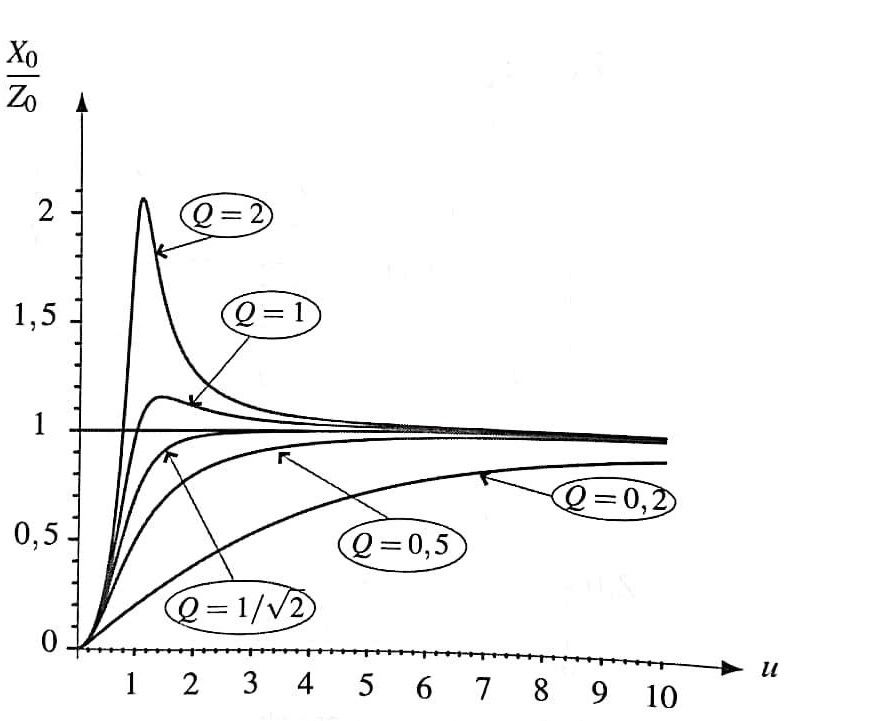
\includegraphics[width=0.45\textwidth]{courbes.jpg}
  \label{fig:maison}
    \caption{Réponse fréquentielle d'un sismographe}
\end{figure}


\item Vérifier que l’allure du graphe sur la figure 4 est compatible, à haute et basse fréquence, avec l’expression calculée. Comment peut-on qualifier ce filtre ? 

\item Comment faut-il choisir la pulsation propre $\omega _0$ par rapport à la pulsation $\omega$ de la secousse
sismique ? Justifier physiquement ce résultat. 

\item Quel est le meilleur choix pour le paramètre $Q$, en terme de fidélité de la réponse et de
durée du régime transitoire ? 
\item Quel est l'ordre de grandeur de l'allongement du ressort à l'équilibre pour un sismographe optimisé pour détecter des ondes sismiques dont la période est de l'ordre de la seconde ? 


\end{enumerate}


\end{document}



\section{Exercice 1}

\section{Exercice 2}

\section{Exercice 3}

\section{ Formulaire }

\end{document}